\subsection{Part a}

There are 3 loops within this DFG. These loops are indicated below:

\begin{figure}[H]
	\centering
	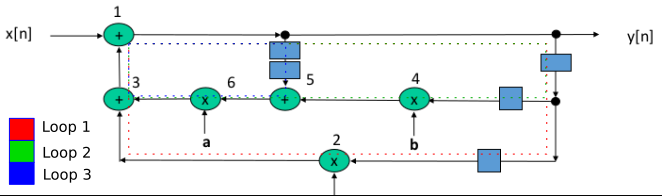
\includegraphics[width=0.8\textwidth]{images/DFGLoop}
	\caption{DFG with Loops labelled}
	\label{fig:images-DFGLoop}
\end{figure}

Each of these loops can be seen to begin and end at the addition node after
the input $x[n]$.
